\documentclass[twoside,a4paper,justified,12pt]{tufte-handout}
\usepackage[greek,spanish,es-tabla]{babel}
\usepackage[utf8]{inputenc}
\usepackage[shortlabels]{enumitem}
%\usepackage[a4paper,top=1.7in,headheight=1.2in]{geometry}
\usepackage{cancel,amsmath,amssymb,amstext,tabularx,chemfig,tikz}
\usetikzlibrary{decorations}
\usepackage{dashrule,tabularx,xcolor,graphicx,fancyhdr,titlesec}
\usepackage{xmpincl}
\usepackage{hyperref}
\includexmp{CC_NC_SA_40}

\pagestyle{fancy}

\setatomsep{2em}

\renewcommand{\headrulewidth}{0pt}

\fancyhead[LO]{
Estructura y enlace
}
\fancyhead[RE]{\scshape{}Àngel Gómez Sicilia}
\fancyhead[LE,RO]{}
\fancyfoot[RE,RO]{\includegraphics[scale=.5]{by-nc-sa.eps} \parbox[b]{.5\textwidth}{Este documento está licenciado bajo Creative Commons 4.0.}}
\cfoot{}
\fancyfoot[LO,LE]{\thepage}

\fancypagestyle{myFirstPage}{%
  \fancyhf{}
  \fancyfoot[RE,RO]{\includegraphics[scale=.5]{by-nc-sa.eps} \parbox[b]{.5\textwidth}{Este documento está licenciado bajo Creative Commons 4.0.}}
  \cfoot{}
  \fancyfoot[LO,LE]{\thepage}
}


%\titleformat{\section}[runin]{\bfseries}{Ejercicio~\thesection.}{1ex}{}[\normalfont]

\setlength{\parindent}{0pt}

\definecolor{not-purple}{HTML}{40ffc0}

\newcommand{\gm}{\greektext{}m\latintext{}}
\newcolumntype{C}{>{\centering\arraybackslash}X}
\newcolumntype{M}[1]{>{\centering\arraybackslash}m{#1}}
\newcolumntype{N}{@{}m{0pt}@{}}
\renewcommand{\sb}[1]{\textsubscript{#1}}
\renewcommand{\sp}[1]{\ensuremath{^{#1}}}

%\newcommand{\bl}[1]{\textcolor{blue}{#1}}
\newcommand{\bl}[1]{\ignorespaces}

\renewcommand{\theenumi}{\alph{enumi}}

\title{Estructura y enlace -- Estructura de Lewis}

\author{Àngel Gómez Sicilia}

\date{Última revisión: \today}

%delocalized bonds chemfig
\pgfdeclaredecoration{ddbond}{initial}{
  \state{initial}[width=4pt]{
    \pgfpathlineto{\pgfpoint{4pt}{0pt}}
    \pgfpathmoveto{\pgfpoint{2pt}{2pt}}
    \pgfpathlineto{\pgfpoint{4pt}{2pt}}
    \pgfpathmoveto{\pgfpoint{4pt}{0pt}}
  }
  \state{final}{
    \pgfpathlineto{\pgfpointdecoratedpathlast}
  }
}
\tikzset{lddbond/.style={decorate, decoration=ddbond}}
\tikzset{rddbond/.style={decorate, decoration={ddbond, mirror}}}


\begin{document}

\shorthandoff{>}\shorthandoff{<}%si no tikz se vuelve loco con babel

\maketitle
\thispagestyle{myFirstPage}

Las moléculas deben su comportamiento químico a la forma por la cual interactúan con otras. Para saber esto, una primera aproximación es la estructura de Lewis, que nos indica qué átomos tienen carga (parcial o total) positiva en la molécula, y cuáles tienen electrones no enlazantes.

Sin embargo, esto no siempre es suficiente: Aunque sepamos qué átomos son más propensos para interactuar con otros, también necesitamos saber dónde se encuentran esos átomos. Para ello es indispensable conocer la posición relativa entre átomos, es decir, la geometría de la molécula.

\section{Hibridación}

Hay múltiples teorías que explican la geometría molecular. Sin embargo, nos centraremos en la más usada hoy en día: la teoría de hibridación de orbitales.

Esta teoría indica que los electrones de valencia de un átomo no se sitúan exclusivamente en el orbital que les toca según la regla de Moeller, sino que en realidad los orbitales de valencia se unen en nuevos orbitales. Por ejemplo, si tenemos un átomo de carbono, la configuración electrónica nos dice que la capa de valencia de este átomo es $2$s\sp{2} $2$p\sp{2}, y podemos hacer una representación en cajas de la misma (v. figura~\ref{fig:carbono_cajas}).

\begin{figure}
    \centering
    \begin{tikzpicture}[scale=.25]
    %   \draw (0,7) rectangle (4,11);
    %   \draw (2,6) node {1s};
    %   \draw[thick, -stealth] (1,8) -- (1,10);
    %   \draw[thick, -stealth] (3,10) -- (3,8);
      %%%%%%%%%%%%%%%%%%%%%%%%%%%%
      \draw (0,0) rectangle (4,4);
      \draw (2,-1) node {2s};
      \draw[thick, -stealth] (1,1) -- (1,3);
      \draw[thick, -stealth] (3,3) -- (3,1);
      %%%%%%%%%%%%%%%%%%%%%%%%%%%%
      \draw (6,0) rectangle (10,4);
      \draw[thick, -stealth] (7,1) -- (7,3);
    %   \draw[thick, -stealth] (9,3) -- (9,1);
      \draw (10,0) rectangle (14,4);
      \draw[thick, -stealth] (11,1) -- (11,3);
    %   \draw[thick, -stealth] (13,3) -- (13,1);
      \draw (12,-1) node {2p};
      \draw (14,0) rectangle (18,4);
    %   \draw[thick, -stealth] (15,1) -- (15,3);
    %   \draw[thick, -stealth] (17,3) -- (17,1);
      %%%%%%%%%%%%%%%%%%%%%%%%%%%%
    %   \draw[black!50] (6,-7) rectangle (10,-3);
    %   \draw[thick, -stealth,black!50] (7,-6) -- (7,-4);
    %   \draw[thick, -stealth,black!50] (9,-4) -- (9,-6);
    %   \draw[black!50] (10,-7) rectangle (14,-3);
    %   \draw[black!50] (12,-8) node {2p};
    %   \draw[black!50] (14,-7) rectangle (18,-3);
    %   \draw[ultra thick,red!50] (5.75,-7.25) -- (18.25,-2.75);
    %   \draw[ultra thick,red!50] (5.75,-2.75) -- (18.25,-7.25);
    \end{tikzpicture}
    \caption{Configuración electrónica de la capa de valencia de un átomo de carbono.}
    \label{fig:carbono_cajas}
\end{figure}

Podemos observar en la figura que el orbital $2$s tiene dos electrones, y que el orbital $2$p tiene a su vez otros dos. Podemos, sin embargo, combinar las cuatro cajas que aparecen en la figura de forma que se consigan otras cuatro distintas, que reduzcan la energía global del átomo. Visto geométricamente, sería la siguiente transformación:

\begin{enumerate}[1)]
    \item En primer lugar estudiamos la capa de valencia de los átomos implicados: La molécula de metano tiene un átomo de carbono y cuatro de hidrógeno.
    \begin{itemize}
        \item El carbono tiene una configuración electrónica \sb{6}C: $1$s$^2$ $2$s$^2$ $2$p$^2$. Su capa de valencia es la $2$, y contiene 2 electrones en el orbital s y 2 en los orbitales p. En total, 4 electrones de valencia.
        \item El hidrógeno tiene una configuración electrónica \sb{1}H: $1$s$^1$. Su capa de valencia es la $1$, en la que tiene 1 electrón.
        \item Tenemos 4 electrones del carbono y 1 electrón por cada hidrógeno, por lo que en total hay 8 electrones disponibles. Podemos representarlos como puntos alrededor de cada átomo.
    \end{itemize}
    
    {\centering{}\chemfig{\lewis{0.,H}}\hspace{2em}\chemfig{\lewis{0.2.4.6.,C}}\\}
    
    \item A continuación elegimos qué átomo deberá ir en el centro de la molécula. Las condiciones que debe cumplir este átomo son las siguientes:
    \begin{itemize}
        \item No puede ser el átomo de hidrógeno.
        \item Debe ser preferentemente el menos electronegativo\footnote{Recuerda que mientras más cercano al flúor en la tabla, más electronegativo. Recuerda también que en lo que a electronegatividad se refiere el hidrógeno está en la parte superior del grupo 15.}.
    \end{itemize}
    Como el átomo central no puede ser el hidrógeno, la única solución posible es que lo sea el carbono.
    
    \item Seguidamente estudiamos el número de electrones que le falta a cada uno. Por ejemplo:
    \begin{itemize}
        \item Para que el carbono complete su capa de valencia hasta 8 electrones y obtenga una configuración estable como el gas noble más próximo (el neón), necesita 4 electrones. Por suerte, tenemos cuatro hidrógenos, cada uno con su electrón y dispuestos a compartirlos.
        \item Igualmente, cada hidrógeno necesitará un electrón para tener 2 en su capa de valencia y ser como el gas noble más próximo (el helio), por lo que usarán los electrones del carbono.
        \item Cada par compartido se pintará con una raya.
    \end{itemize}
    
     {\centering{}\chemfig{H-C(-[2]H)(-[6]H)-H}\\}
    
\end{enumerate}

Esta sería la estructura de Lewis del metano.

Veamos otros ejemplos:

\subsection{Molécula con electrones no enlazantes}

La molécula de agua, H\sb{2}O, está compuesta por dos oxígenos y un hidrógeno.

\begin{enumerate}[1)]
    \item La configuración electrónica de sus elementos es
    \begin{itemize}
        \item \sb{8}O: $1$s$^2$ $2$s$^2$ $2$p$^4$.
        \item \sb{1}H: $1$s$^1$.
    \end{itemize}
    
    Tiene en total 10 electrones de valencia, y su diagrama con puntos sería como sigue.
    
    {\centering{}\chemfig{\lewis{0.,H}}\hspace{2em}\chemfig{\lewis{0:2:4.6.,O}}\\}
    
    \item En este caso el átomo central no podrá ser el hidrógeno, por lo que tiene que ser el oxígeno.
    
    \item Finalmente observamos que el oxígeno necesita 2 electrones, que tomará 1 de cada hidrógeno:
        
     {\centering{}\chemfig{H-\lewis{0:2:,O}-[6]H}\\}
     
    \item Fíjate en que la estructura de Lewis es una representación esquemática de los enlaces sin tener en cuenta la geometría molecular. Por este motivo, la estructura del agua es válida en estas otras formas también:
    
    {\centering{}\chemfig{H-\lewis{0:6:,O}-[2]H}\hspace{2em}\chemfig{\lewis{4:6:,O}(-[2]H)-H}\hspace{2em}\chemfig{\lewis{4:2:,O}(-[6]H)-H}\hspace{2em}\chemfig{H-\lewis{2:6:,O}-H}\hspace{2em}\chemfig{\lewis{4:0:,O}(-[2]H)-[6]H}\\}
    
    \item Además, los electrones que no enlazan en ocasiones también se pone con una línea en lugar de puntos, es equivalente \chemfig{\lewis{6:2:,O}(-[4]H)-H} que \chemfig{\lewis{62,O}(-[4]H)-H}
    
\end{enumerate}

\subsection{Molécula con enlaces dobles}

El caso del O\sb{2} es ligeramente distinto. Veámoslo:

\begin{enumerate}[1)]
    \item La configuración electrónica de sus elementos es
    \begin{itemize}
        \item \sb{8}O: $1$s$^2$ $2$s$^2$ $2$p$^4$.
    \end{itemize}
    
    Tiene en total 12 electrones de valencia.
    
    \item Al haber solamente dos átomos, ninguno de ellos es el central.
    
    \item A cada oxígeno le faltan dos electrones para completar el octeto. No sería suficiente con un enlace entre ellos. Además, un único enlace dejaría electrones sin pareja (\hspace{1ex}\chemfig{\lewis{4:2:6.,O}-\lewis{0:2:6.,O}}\hspace{1ex}). Por este motivo, los dos oxígenos comparten, cada uno, dos electrones y forman así un \textit{enlace doble}.
        
     {\centering{}\chemfig{\lewis{5:3:,O}=\lewis{7:1:,O}}\\}
     
     \item Contando observamos que cada oxígeno tiene 4 electrones no-compartidos y 4 compartidos, 8 en total.
     
\end{enumerate}

\subsection{Molécula con enlaces triples}

El caso del N\sb{2} es parecido al anterior.

\begin{enumerate}[1)]
    \item La configuración electrónica de sus elementos es
    \begin{itemize}
        \item \sb{7}N: $1$s$^2$ $2$s$^2$ $2$p$^3$.
    \end{itemize}
    
    Tiene en total 10 electrones de valencia.
    
    \item Al haber solamente dos átomos, ninguno de ellos es el central.
    
    \item A cada nitrógeno le faltan tres electrones para completar el octeto. A pesar de que en este caso un enlace no deja electrones despareados (\hspace{1ex}\chemfig{\lewis{4:2:,N}-\lewis{0:2:,N}}\hspace{1ex}), ni un enlace simple ni uno doble son suficientes para completar el octeto. Cada nitrógeno comparte tres electrones y forman así un \textit{enlace triple}.
        
     {\centering{}\chemfig{\lewis{4:,N}~\lewis{0:,N}}\\}
     
     \item Contando observamos que cada nitrógeno tiene 2 electrones no-compartidos y 6 compartidos, 8 en total.
\end{enumerate}

\subsection{La regla VTEN}

La mayoría de compuestos covalentes tienen una estructura de Lewis sencilla y se puede usar un método para representarla. Este método consiste en calcular el número de electrones de valencia ($V$), el número total de electrones necesarios ($T$), y a partir de ellos el número de electrones enlazantes ($E$) y el número de electrones no-enlazantes ($N$). Veamos cómo se aplica con un ejemplo, el CO\sb{2}.

\begin{enumerate}[1)]
    \item En primer lugar estudiamos la configuración electrónica de cada elemento.
    \begin{itemize}
        \item \sb{6}C: $1$s$^2$ $2$s$^2$ $2$p$^2$.
        \item \sb{8}O: $1$s$^2$ $2$s$^2$ $2$p$^4$.
    \end{itemize}
    
    En la capa de valencia tienen 4 y 6 electrones, respectivamente. En total hay $4+6\cdot2=16$~electrones. Por tanto, $V=16$.
    
    \item Cada átomo necesita 8 electrones para completar el octeto (menos el hidrógeno que necesita 2). Como esta molécula tiene 3 átomos y ninguno es hidrógeno, necesitamos $8\cdot 3=24$~electrones. Por tanto, $T=24$.
    
    \item Los electrones que comparte cada átomo son los que le faltan para llegar al total, por lo que los electrones enlazantes son $E=T-V$, que en este caso es $E=8$. Como normalmente interesan más los pares, diremos que tenemos 4~pares enlazantes.
    
    \item El resto de electrones no formarán ningún enlace, por lo que $N=V-E$, que en este caso será $N=8$, también 4~pares no-enlazantes.
    
    \item Cuando tenemos $E$ y $N$, simplemente colocamos los átomos como de costumbre, con el menos electronegativo en el centro (menos el hidrógeno, que no puede ser el del centro), y ponemos los pares enlazantes. En este caso el carbono irá en el centro, y dado que hay 4~pares enlazantes para 2 enlaces pondremos 2 enlaces dobles.
    
     {\centering{}\chemfig{O=C=O}\\}
     
    \item Finalmente contamos los electrones en cada átomo, y a aquellos átomos que les falten electrones para completar el octeto les añadimos pares no enlazantes. El carbono tiene 4~electrones compartidos con cada oxígeno, en total 8~electrones, por lo que no admite más. Cada oxígeno, sin embargo, tiene solamente los 4 que comparte con el carbono, por lo que necesitará otros 4 para alcanzar el octeto. La molécula queda
    
      {\centering{}\chemfig{\lewis{3:5:,O}=C=\lewis{1:7:,O}}\\}
      
    \item Observa que si cuentas los electrones de cada átomo salen 8, por la regla del octeto; y si cuentas el número total de electrones sale 16, que son los electrones que tenemos ($V$).
    
\end{enumerate}

\subsection{Moléculas con tres elementos}

Un caso interesante es el ácido cianhídrico, HCN. Este compuesto tiene tres átomos.

\begin{enumerate}[1)]
    \item Como de costumbre, primero hacemos la configuración electrónica de cada elemento.
    \begin{itemize}
        \item \sb{1}H: $1$s$^1$.
        \item \sb{6}C: $1$s$^2$ $2$s$^2$ $2$p$^2$.
        \item \sb{7}N: $1$s$^2$ $2$s$^2$ $2$p$^3$.
    \end{itemize}
    
    En la capa de valencia tienen 1, 4 y 5 electrones, por lo que $V=10$.
    
    \item El hidrógeno necesita 2 electrones y el resto necesitan 8, así que $T=18$.
    
    \item Los electrones enlazantes son $E=T-V=8$, 4~pares enlazantes.
    
    \item Los electrones no enlazantes son $N=V-E=2$, 1~par no-enlazante.
    
    \item El átomo menos electronegativo es el carbono, que será el central. Tenemos que poner 4 enlaces, pero si hacemos como antes y ponemos 2 y 2 tendremos un hidrógeno con 4 electrones, le sobran. Por tanto pondremos un único enlace al hidrógeno y el resto, tres, al nitrógeno
    
     {\centering{}\chemfig{H-C~N}\\}
     
    \item Contando observamos que el hidrógeno tiene 2~electrones (y necesita 2, bien), el carbono tiene 8 electrones (bien) y el nitrógeno tiene 6. Aprovechamos el par no enlazante para completar el octeto del nitrógeno y la molécula final es
    
      {\centering{}\chemfig{H-C~\lewis{0:,N}}\\}
      
    \item Observa que si cuentas los electrones del hidrógeno salen 2, y del carbono y del nitrógeno salen 8, por la regla del octeto; y si cuentas el número total de electrones sale 10, que son los electrones que tenemos ($V$).
    
\end{enumerate}

\subsection{Estructuras resonantes}

Veamos el caso del SO\sb{2}:

\begin{enumerate}[1)]
    \item Configuración electrónica:
    \begin{itemize}
        \item \sb{8}O: $1$s$^2$ $2$s$^2$ $2$p$^4$.
        \item \sb{16}S: $1$s$^2$ $2$s$^2$ $2$p$^6$ $3$s$^2$ $3$p$^4$.
    \end{itemize}
    
    En la capa de valencia todos tienen 6 electrones, por lo que $V=18$.
    
    \item Necesitan 8, así que $T=24$.
    
    \item Los electrones enlazantes son $E=T-V=6$, 3~pares enlazantes.
    
    \item Los electrones no enlazantes son $N=V-E=12$, 6~pares no-enlazantes.
    
    \item El átomo menos electronegativo es el azufre, que será el central. Ahora hay tres pares para dos enlaces, uno de los oxígenos debe ser ``más importante'' que el otro y recibir el enlace doble. Supongamos que es el de la derecha.
    
     {\centering{}\chemfig{O-S=O}\\}
     
    \item Al contar vemos que faltan 6~electrones al oxígeno de la izquierda, 2~al azufre y 4 al oxígeno de la derecha, en total 12 que son los pares no enlazantes (bien). Nos queda
    
      {\centering{}\chemfig{\lewis{2:4:6:,O}-\lewis{2:,S}=\lewis{1:7:,O}}\\}
      
    \item Esta estructura es correcta, pero el oxígeno de la derecha no es más importante que el de la izquierda, por tanto podría ocurrir que los electrones no enlazantes del oxígeno izquierdo pasen a hacer un doble enlace y los del doble enlace de la derecha pasen al oxígeno derecho:
    
    {\centering
    \schemestart
        \chemfig{@{O1}\lewis{2:4:6:,O}-[@{sb}]@{S}\lewis{2:,S}=_[@{db}]@{O2}\lewis{1:7:,O}}
        \arrow{<->}
        \chemfig{\lewis{3:5:,O}=\lewis{2:,S}-\lewis{0:2:6:,O}}
    \schemestop
    \chemmove{% change the tip style
    \draw[->,shorten <=2pt](O1)..  controls +(90:5mm) and +(90:5mm)..  (sb);
    \draw[->,shorten >=1pt](db) ..  controls +(90:6mm) and +(90:4mm) ..  (O2);}\\
    }
    
    \item Ambas estructuras son equivalentes, por lo que no podemos estar seguros de cuál es la correcta. De hecho experimentalmente se observa que ninguna de ellas es la correcta, sino que es una mezcla en la que parece que ambos enlaces estén entre el simple y el doble. Por este motivo, se dice que estas son estructuras resonantes y se representan así:
    
    {\centering
    \schemestart
        \chemleft[\subscheme{
        \chemfig{@{O1}\lewis{2:4:6:,O}-[@{sb}]@{S}\lewis{2:,S}=_[@{db}]@{O2}\lewis{1:7:,O}}
        \arrow{<->}
        \chemfig{\lewis{3:5:,O}=\lewis{2:,S}-\lewis{0:2:6:,O}}
        }\chemright]
    \schemestop\\
    }
    
    o así:    
    
    {\centering \setatomsep{2.5em}\chemfig{\lewis{3:5:,O}-[,,,,lddbond]\lewis{2:,S}-[,,,,lddbond]\lewis{1:7:,O}}\\}
    
\end{enumerate}

Si nos fijamos en una de las estructuras resultantes, por ejemplo en \hspace{2ex}\chemfig{\lewis{2:4:6:,O}-\lewis{2:,S}=\lewis{1:7:,O}}\hspace{2ex}, observaremos que el oxígeno que hay a la izquierda tiene 6 electrones sin compartir. Si vamos al principio del ejercicio, en la configuración electrónica, veremos que originalmente el oxígeno tenía 6 electrones de valencia. Esto significa que el oxígeno forma parte de esta molécula sin compartir ningún electrón. Si marcamos los electrones de cada átomo por el color, observamos lo siguiente:\\[1ex]

 {\centering{}
 \schemestart
   \chemfig{\setlewis{}{}{orange}\color{orange}\lewis{2:4:6:0.,O}-%
   \setlewis{}{}{}\lewis{2:4.0:,S}=%
   \setlewis{}{}{blue}\color{blue}\lewis{4:1:7:,O}}
 \schemestop
 \chemmove{% change the tip style
 \fill[black] (-1.34,0.125) circle (.2ex);}\\[2ex]}

Observamos que uno de los enlaces se forma con dos electrones del azufre, que es ``generoso'' y comparte los dos para que el oxígeno, que es ``egoísta'' y no comparte, llegue al octeto. Este tipo de enlace se llama \textit{enlace dativo} o \textit{enlace de coordinación} y suele venir acompañado por resonancia. El enlace dativo se representa con una flecha:\\[1ex]


 {\centering{}
 \schemestart
   \chemfig{@{O}\lewis{2:4:6:,O}-@{S}\lewis{2:,S}=\lewis{1:7:,O}}
 \schemestop
 \chemmove{% change the tip style
 \draw[shorten >=1pt, shorten <=1pt] (S) -- (O);}\\[2ex]}

Otro ejemplo de estructura resonante que también tiene enlaces dativos sería el ácido nítrico, HNO\sb{3}:

\begin{tabularx}{.95\textwidth}{cC}
$\begin{array}{rl}
    V&=12\\
    T&=18\\
    E&=6\\
    N&=6
\end{array}$
&

    {\centering
    \schemestart
        \chemleft[\subscheme{
        \chemfig{@{N1}N(-[3]@{O1}\lewis{1:3:5:,O})(-[1]\lewis{1:3:,O}-[7]H)=[6]\lewis{5:7:,O}}
        \arrow{<->}
        \chemfig{@{N2}N(=[3]\lewis{2:4:,O})(-[1]\lewis{1:3:,O}-[7]H)-[6]@{O2}\lewis{0:4:6:,O}}}
        \chemright]
    \schemestop
 \chemmove{% change the tip style
 \draw[shorten >=1pt, shorten <=1pt] (N1) -- (O1);
 \draw[shorten >=1pt, shorten <=1pt] (N2) -- (O2);}\\
    }
    
\end{tabularx}


\section{Octeto incompleto y octeto expandido (Ampliación)}

En algunos compuestos hay elementos que no cumplen la regla del octeto, ya sea por defecto o por exceso de electrones. Para estos compuestos no se puede usar la regla VTEN para hacer su estructura de Lewis, sino que se debe hacer por tanteo. Veamos un ejemplo de cada caso:

El octeto expandido se da con elementos a partir del periodo 3. Esto es debido a que en este nivel y superiores existe el orbital d, que también admite electrones, mientras que el nivel 2 no lo tiene. Es muy típico encontrar este tipo de configuración con el fósforo o el azufre como átomos centrales, y es fácil de identificar porque al usar la regla VTEN nos salen menos enlaces de los que necesitamos. Por ejemplo, veamos el PCl\sb{5} y el H\sb{2}SO\sb{4} (ver tabla~\ref{tab:excepciones}).

Otros compuestos sufren del efecto contrario, algunos de sus elementos se conforman con menos de 8 electrones para que sus compañeros de molécula puedan tener los 8. Los átomos que se quedan con menos de 8 electrones tienen \textit{octeto incompleto} y pueden ser solamente elementos bastante poco electronegativos, como el berilio, el boro o el aluminio. El BeO y del BF\sb{3} son ejemplos de moléculas con octeto incompleto (ver tabla~\ref{tab:excepciones}). 

\begin{table}[bp]
\begin{tabularx}{.95\textwidth}{cC}

    \multicolumn{2}{c}{\scshape Octeto expandido}\\\hline\\[1ex]
$\begin{array}{rl}
    V&=40\\
    T&=48\\
    E&=8\\
    N&=32
\end{array}$
&
    \chemfig{P(-[2]\lewis{0:2:4:,Cl})(-[::162]\lewis{2:4:6:,Cl})(-[::234]\lewis{3:5:7:,Cl})(-[::306]\lewis{1:5:7:,Cl})-[::18]\lewis{0:2:6:,Cl}}\\
    \multicolumn{2}{p{.9\textwidth}}{Salen 8~electrones enlazantes, que son 4 enlaces, pero necesitamos 5 porque hay 5 Cl.}\\ \hline\\[1ex]
$\begin{array}{rl}
    V&=32\\
    T&=44\\
    E&=12\\
    N&=20
\end{array}$
&
   \chemfig{S(=[2]\lewis{1:3:,O})(=[6]\lewis{5:7:,O})(-[4]\lewis{2:6:,O}-[4]H)-[0]\lewis{6:2:,O}-[0]H}\\
    \multicolumn{2}{p{.9\textwidth}}{Nos salen 12 electrones enlazantes, 6 pares. Se podrían enlazar los átomos con 6 pares (uno para cada \chemfig{S-O} y uno para cada \chemfig{O-H}) y el azufre cumpliría la regla del octeto, pero los oxígenos no la podrían cumplir, y como el oxígeno es más electronegativo es mejor que el oxígeno la cumpla aunque el azufre se pase de 8.}\\ \hline\hline
    \multicolumn{2}{c}{\scshape Octeto incompleto}\\\hline\\[1ex]
$\begin{array}{rl}
    V&=8\\
    T&=16\\
    E&=8\\
    N&=0
\end{array}$
&
    \chemfig{Be=\lewis{2:6:,O}}\\
    \multicolumn{2}{p{.9\textwidth}}{Salen 8~electrones enlazantes, que son 4 enlaces, pero como el oxígeno es muy electronegativo prefiere tener los enlaces para sí mismo.}\\ \hline\\[1ex]
$\begin{array}{rl}
    V&=24\\
    T&=32\\
    E&=8\\
    N&=16
\end{array}$
&
   \chemfig{B(-[2]\lewis{4:2:0:,F})(-[7]\lewis{1:7:5:,F})-[5]\lewis{5:3:7:,F}}\\
    \multicolumn{2}{p{.9\textwidth}}{Este caso es muy claro, como el flúor es halógeno y nunca puede formar enlaces dobles, al boro no le queda más remedio que conformarse con 3 enlaces (6 electrones) aunque en la regla VTEN nos salgan 8.}\\ \hline
    
\end{tabularx}
\caption{Ejemplos de octeto expandido e incompleto.}
\label{tab:excepciones}
\end{table}


\end{document}